\chapter{The Atacama Cosmology Telescope: point source analysis of beams for DR6}
\label{ch:actbeams}

\section{\label{sec:act_intro}Introduction}
\setcounter{footnote}{0}

The Atacama Cosmology Telescope (ACT) is a 6\,m off-axis Gregorian telescope located at an altitude of 5190\,m in the Atacama Desert of northern Chile. It is designed for millimeter wavelength observations of the cosmic microwave background (CMB) at arcminute resolution.  The telescope and receiver are described in \cite{fowler_2007} and \cite{thornton_2016} respectively. 

This paper describes an alternative method for determining the optical response of the telescope based on stacking point source observations.  This data release includes temperature and polarization data collected by ACT between 2017 and 2021, covering roughly 18,000 square degrees of the sky~\cite{thornton_2016}.

Determining the optical response, or "beam", quantifies how the instrumental response is suppressed at small angular scales as a result of the finite resolving power of the optics.  For this reason, understanding the telescope beam and its uncertainty is critical for achieving the science goals of ACT.  Because the beam has to be de-convolved from the sky maps in order to perform cosmological analysis, incorrectly characterizing the beam directly biases any science by mimicking a spurious scale-dependent signal.  Therefor, in order to achieve the science goals set out by ACT, characterization of the instrument beam is crucial.  Besides the beam of the instrument, it is also important for a polarimetric instrument like ACT to quantify the amount of temperature-to-polarization leakage. We describe this type of leakage in terms of a so-called "leakage beam", quantifies the amount of leaked signal from Stokes I to Stokes Q or U at a given angular scale.

Previous work to characterize the ACT instrument beam have done so with planet maps (~\cite{hasselfield_atacama_2013,louis_2017,naess_2014}).  Planets served as the best candidates for beam characterization of the telescope~\cite{Lungu_2022}.  Specifically, observations of Uranus achieve adequate signal-to-noise without exceeding the dynamic range of the instrument.  Here, we present a novel technique to characterize the instrument beam with map data, which we refer to as "stacking" of the point-sources in a map's catalog.  This work provides a detailed recipe for characterizing an instrument's beam using full map data, which we apply to the ACT DR6 maps.  This method provides a validation of the Uranus-derived beam both in temperature $T$ and in the $T\rightarrow E$ and $T\rightarrow B$ leakage.  Such a novel validation is necessary because the Uranus observations are separate observations made with a different strategy than the full maps, have different noise properties and were made using a different map-making technique.  The point-source stacking method, presented here, uses the same observations which we use for cosmology, thus providing a check to the beam and leakage inferred from Uranus observations.

\begin{figure*}[t]
\vspace{1em}
    \centering
    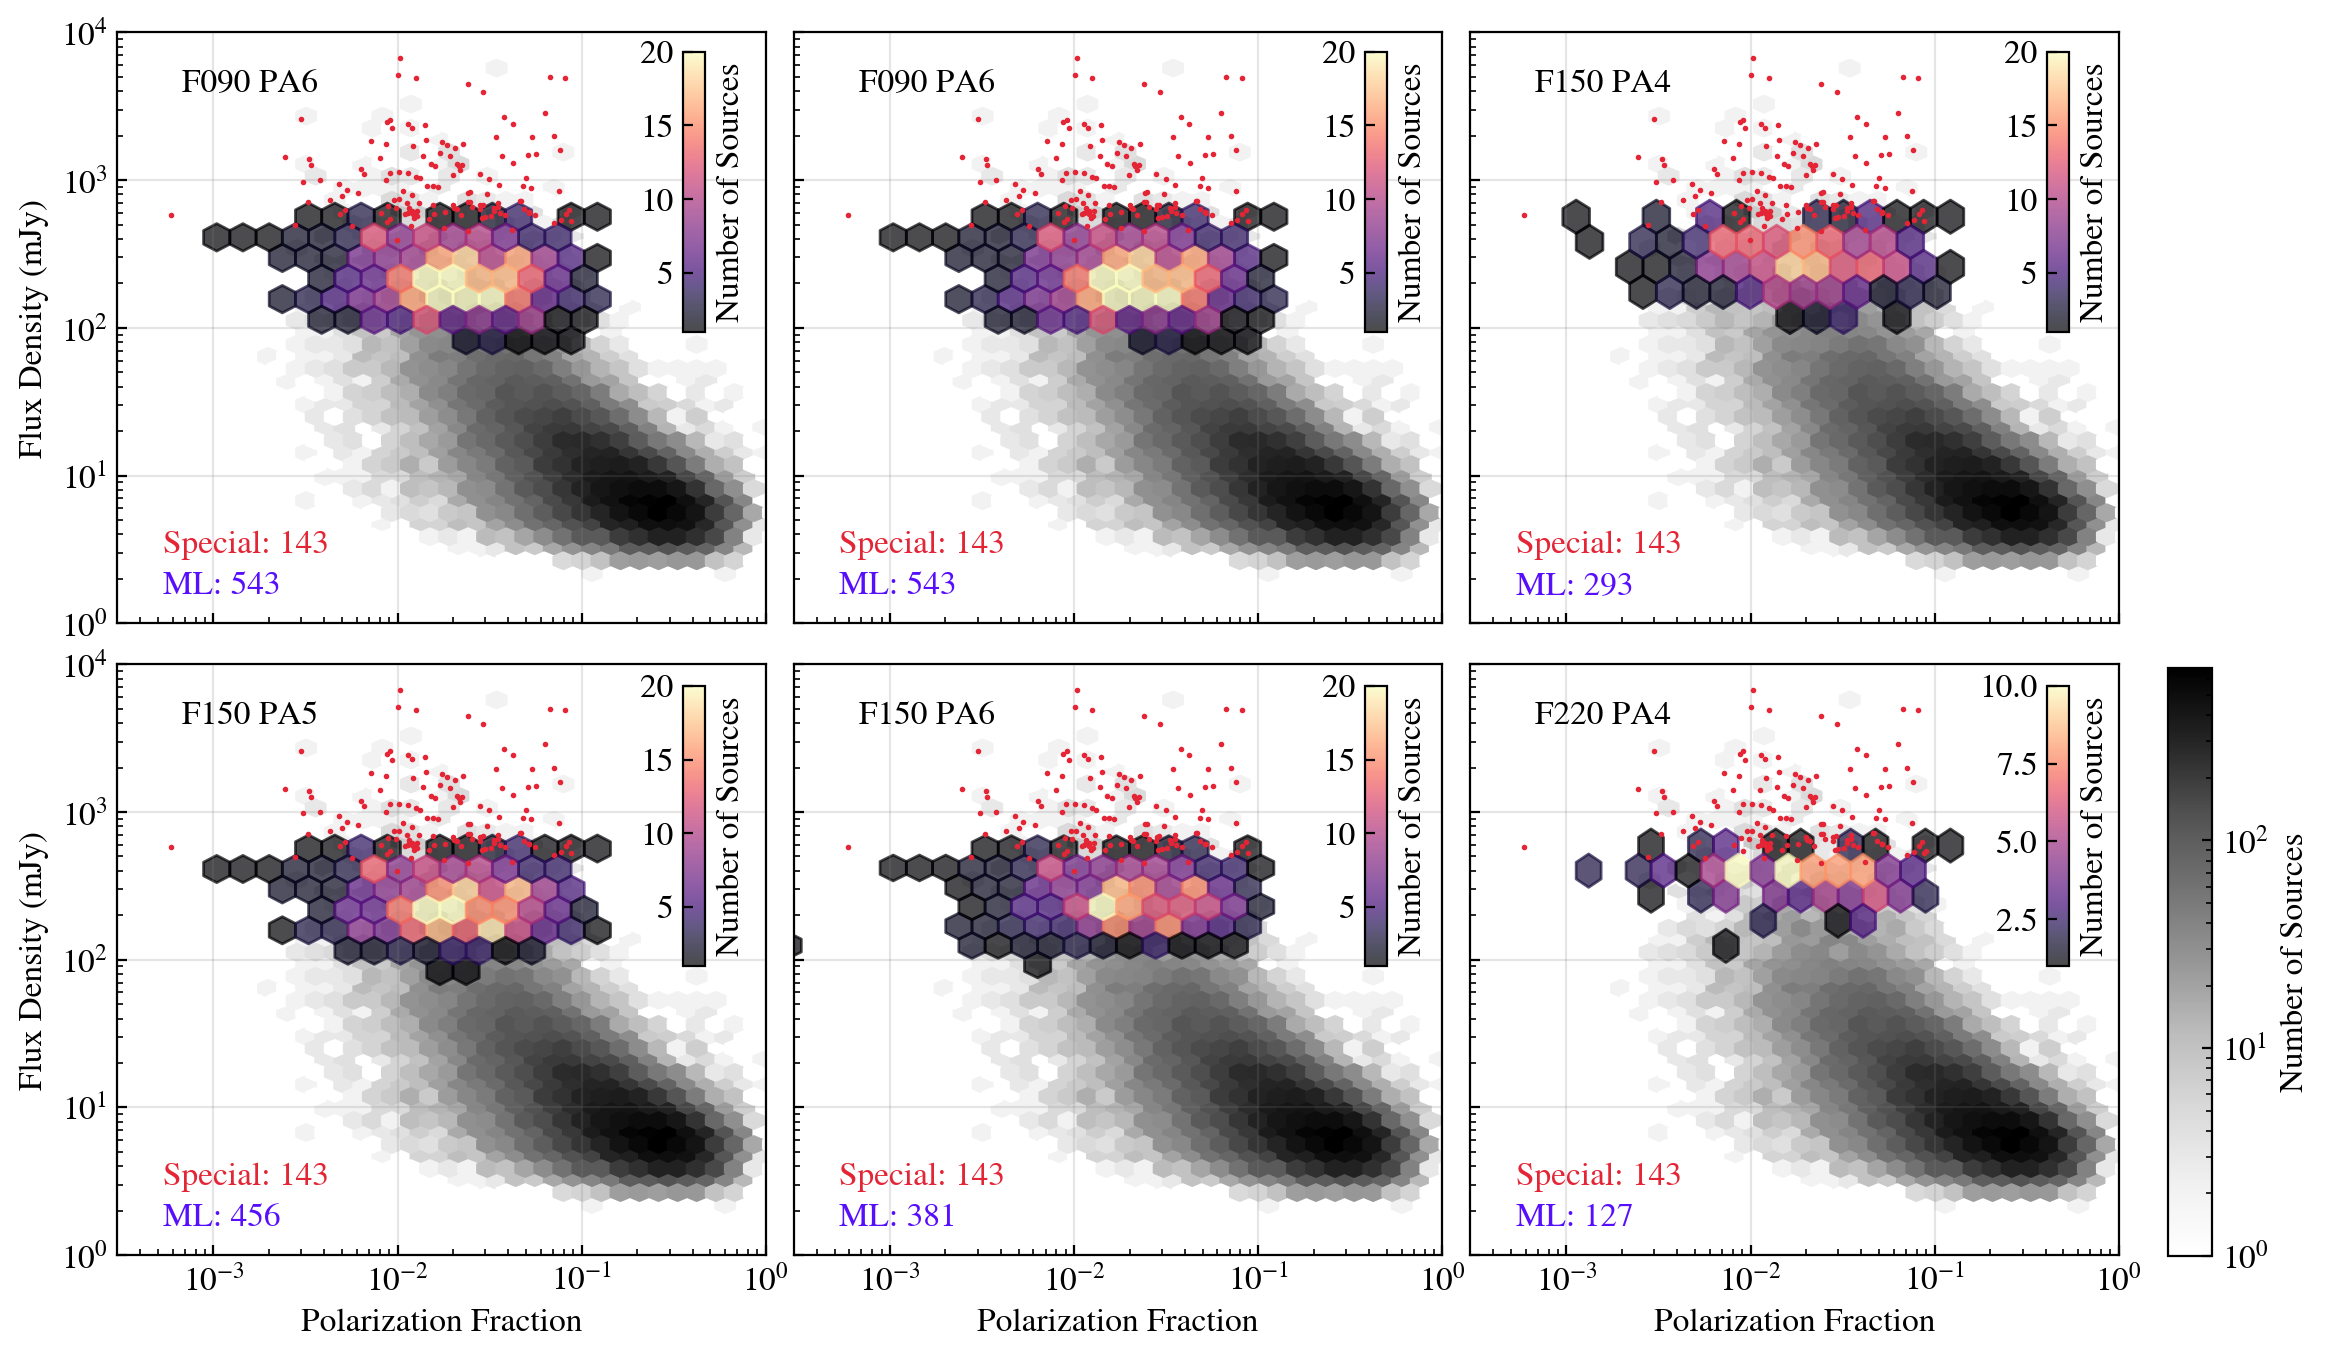
\includegraphics[width=\linewidth]{Figures/pt_src_dist.png}
    \caption{Distribution of the total number of point sources that were in the catalog (faded colors) and ultimately became part of the final beam analysis (solid colors) for all arrays combined, shown by observing seasons from 2017--19.
    }
    \label{fig:ptsrc_select}
    \vspace{1em}
\end{figure*}

The paper is organized as follows. 
In \S\ref{sec:obs} we describe the observations and catalog used to stack point sources and characterize the ACT beams.  In \S\ref{sec:stack} we explain the stacking process, starting from an input map and producing a stacked beam profile.  In \S\ref{sec:sim_pipe} we describe the steps of the map simulation pipeline, then going from simulated point-source maps to a model of the ACT beams and their covariance.  In \S\ref{sec:act_results} we present the results from the stacking method, including the stacked temperature to polarization leakage, and the temperature beam radial profiles.  Finally, in \S\ref{sec:act_disc} we discuss assumptions made in the analysis and future directions for ACT beam characterization.

\begin{figure*}[t]
    \centering
    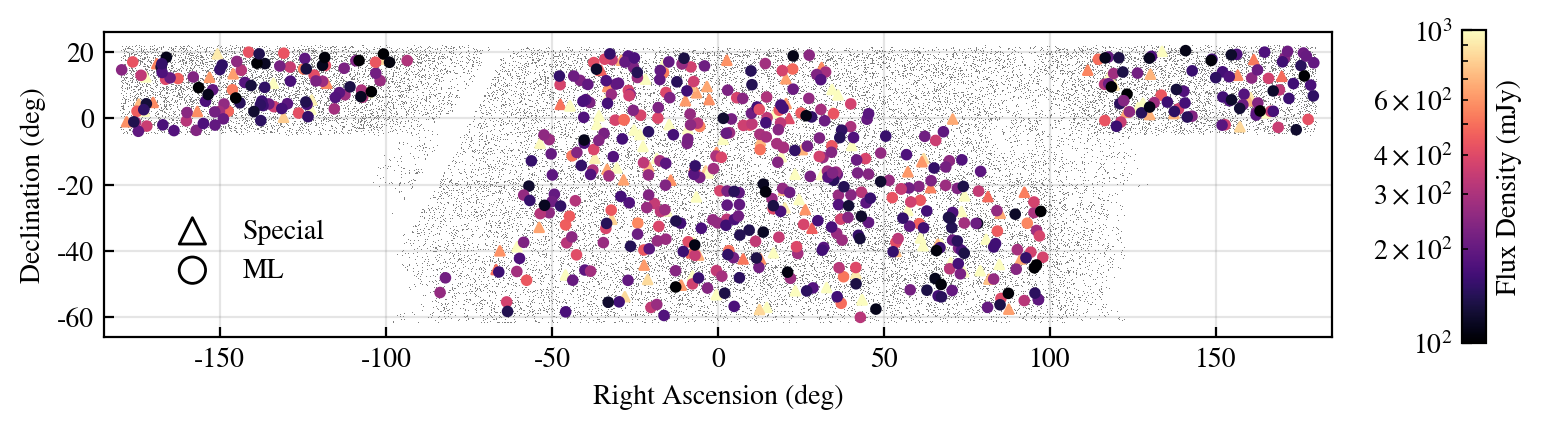
\includegraphics[width = \textwidth]{Figures/ptsrc_map.png}
    \caption{Spatial distribution of point sources from catalog(grey) and used in stacking(colored).  The color bar shows the flux of the special(ML) sources, which are plotted as triangles(circles).}
    \label{fig:ptsrc_map}
\end{figure*}

\section{Observations}
\label{sec:observations}

The  data used in this work are part of the upcoming 6th data release (DR6) of ACT. DR6 consists of observation taken between 2017 and 2021 using three dichroic detector arrays, PA4, observing using broad frequency passbands roughly centered on  150 and 220\,GHz, and PA5 and PA6, both with passbands centered on 98 and 150\,GHz. The 3 types of frequency bands are referred to by f090, f150 and f220. On the sky, the observations fall in to the "Advanced Act" region as defined in \cite{aiola_2020}, which includes roughly 45\% of the full sky. The observations are taking during both day and night; in this work, we restrict ourselves to the nighttime data, as this subset of the data is the current focus of the cosmological analysis performed by the ACT collaboration. The DR6 data and analyses have not been made public yet at the time of writing.

The DR6 data are divided into 8 non-overlapping subsets and mapped into sky maps. In this work, we only use co-added versions of these 8 maps. We thus consider a single triplet of Stokes I, Q and U maps for each of the 6 combinations of PA4/5/6 and their two frequency bands. 

The maps are produced in the Plate-Carr\'{e}e cylindrical projection (CAR) using a maximum-likelihood (ML) technique that is described in \cite{aiola_2020}. There is one exception, which is relevant for this work: the brightest point sources are mapped with a specialized source mapmaker. This special treatment of bright point sources is needed because the ML mapmaker produces artifacts when mapping bright localized sources, see \cite{naess_2019} for a detailed explanation. In the DR6 maps, the specialized mapmaker is used for a pre-selected set of bright sources. We will refer to the bright sources that underwent this specialized treatment as "special" sources, while we refer to the fainter sources that were mapped using the regular mapmaker as "ML" sources.

\section{Methods}
\label{sec:stack}
Here we walk through the stacking process from input map to beam profile.  
\subsection{Point-source Selection}
\label{subsec:ptsrc_sel}
Prior to stacking, we characterize each point source to determine whether they are suitable for stacking.  The number of point sources used for the point source analysis versus the total number of point sources in the catalog is shown in Figure~\ref{fig:ptsrc_select}.

\subsubsection{Select on Catalog}
\label{subsubsec:cat_sel}
For ease of interpretation, a sky mask is applied that is similar to those used by the various cosmological analysis. This mask removes regions with strong Galactic emission (based on the 353 GHz Planck data) and significantly noisy regions on the sky.  The point source catalog has been estimated from the DR6 maps using a matched filter approach. Through the use of the 3 ACT frequency bands, the catalog also includes an estimate of the type of each source (synchrotron, flat or dusty spectrum, as well as SZ clusters). The catalog will be described in forthcoming publications accompanying the DR6 release.

From the catalog, we obtain a list of RA's and DEC's of point-sources in the map.  However, it is not a given that each point-source from the catalog appears on our map, so we reject any coordinates which fall outside the boundary of the input map $\mathbf m$.  Additionally, we select only point synchrotron sources, such that we stack over individual point sources rather than galaxy clusters, rather than dusty galaxies or galaxy clusters.  The brightest sources are synchrotron sources; so these cuts do not significantly reduce signal-to-noise.  Rather, this cut simplifies the analysis by removing extended sources while we avoid stacking on sources with different spectral energy densities (and associated differences in optical response).

When stacking point sources, we restrain the point sources to a polarization fraction of below 10\% such that we are not dominated by highly polarized sources.  One would expect the polarization signal to intrinsically average out over the sources' random polarization angles.  However, this is not the case when a few of the brightest sources are strongly polarized and dominate the stack due to inverse-variance weighting (see Sec~\ref{subsubsec:beamqual_sel}), which up-weights sources with the highest signal-to-noise ratios.  Once the selection is complete, the geometry of the stamp is defined to be $40^{\prime}$($30^{\prime}$) wide at a $0.15^{\prime}(0.05^{\prime})$ resolution for the F090 and F150(F220) bands.  The region must be large enough such that the stamp will include side-lobes features, but resolved enough to make out the main beam profile.

\subsubsection{Select on Beam Quality}
\label{subsubsec:beamqual_sel}
With the list of point-source locations on our map from the catalog, we further decide which point-sources to use in the stamp based on a stamp's individual features.  For example, we don't want to include a stamp with two point-sources, or an off-center point-source, in the stack.  To characterize the quality of a point source, each point-source is re-projected to the same geometry (as specified in the last paragraph).  A point source $p_i$ is first peak-normalized.  If the location of its highest peak, $p_{i,1}$, is outside a radius of $0.5^{\prime}$, $p_i$ is assumed to be off-centered and is discarded.  

We next want to determine if the stamp has two point-sources or just one.  To do so, we find the second-highest amplitude in the stamp and assume this to be the second peak, $p_{i,2}$.  If the amplitude of $p_{i,2}$ is within 10\% of the average stamp value (outside the radius $r=\frac{2}{3}r_{\text{FWHM}}$), it is assumed to be dominant, and the point source $p_i$ is discarded.

Figure~\ref{fig:ptsrc_select} shows the number of point sources used in each band and PA from the catalog.  We note that the F090 map stacks included the greatest number of point sources, since the beams are larger and therefore take up a larger area of the stamp's area.  Because the F220 beams are much smaller in beam width, we constrain stamps in this band to a radius of $15^{\prime}$, while the F090 and F150 stamps are at a radius of $30^{\prime}$.

\subsubsection{Special vs. ML Sources}
\label{subsubsec:type_sel}
We subdivide the remaining point sources into two categories: Special and Max-Likelihood (ML) point sources.  When making the maps, as described in Section~\ref{sec:observations}, point sources are treated with the two differing methods, and thus we want to consider the two groups individually when stacking to note any differences this treatment may have caused.  The final distribution of selected point sources is shown in Figure~\ref{fig:ptsrc_select}.

\begin{figure*}[t]
    \centering
    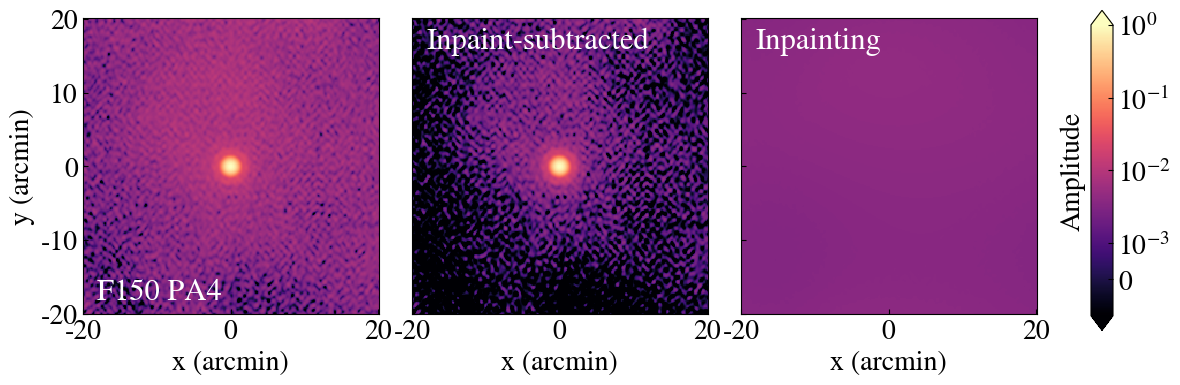
\includegraphics[width=\textwidth]{Figures/inpainting.png}
    \caption{Example inpainting-subtracted method for F150 PA4.  Top: PAX F090 beam and Bottom: PAX F150 beam...}
    \label{fig:example_maps}
    \vspace{1em}
\end{figure*}

\subsection{Stacking}
\label{subsec:stacking}
This section describes the stacking procedure with the selected sources.  Each stamp $s_i$ is re-projected to the same geometry prior to stacking.  Each stamp is cut from the map and re-projected to a tangent plane using a bi-cubic interpolation.  Re-projecting to a tangent plane ensures stacking multiple sources from different declinations are not stretched by different amounts (as a result of the CAR pixelization of the input map).  The bicubic interpolation introduces a small bias resembling a low-pass filter, which we investigate in Section~\ref{sec:sim_pipe}.  We will show this bias is small enough to neglect.

%Because we want our final product to be the beam of the telescope, we employ a large-scale structure removal procedure such that all we are left with is the beam.  First, we use a method we call "inpainting".  
Before stacking the reprojected stamps, we subtract an estimate of the large-scale correlated noise component of the stamp. The correlated noise, coming mainly from the CMB and atmosphere, is relatively bright compared to the point sources (at around the -20 dB level for even the brightest point sources), making it crucial to remove it prior to stacking.  If left in the stamps, the correlated noise is not averaged down enough during stacking as a result of the small number of high signal-to-noise sources in the stack. The resulting stacks show a large amount of noise variance that prohibits measurements of the non-central parts of the beam. We only perform the subtraction on the Stokes $I$ component of the stamps, the Stokes $Q$ and $U$ components have a relatively small amount of correlated noise, making the subtraction procedure unnecessary.

We refer to the subtraction method as ``inpaint-subtraction''. This procedure masks a region centered on the point source and fills this area with a prediction of large-scale correlated noise using only information from the outer area of the stamp. This inpainted region is then subtracted from the original stamp, resulting in a map of the point source with substantially reduced large scale correlated noise. The inpainting is done with a simplified version of the method described in~\cite{bucher_2012}. In short: the method uses the conjugate-gradient method~\cite{Shewchuk_1994} to solve for $s_l$ in:
\begin{equation}\label{eq:inpaint}
\left(S^{-1} + M^{-1} \right) s_l = M^{-1} s
\end{equation}
Here, $s$ denotes the input stamp and $S^{-1}$ denotes the covariance matrix of the correlated noise, modelled as a ``$1/f$'' spectrum in harmonic space: $1/ (1 + \ell / \ell_{\mathrm{knee}}^{-3})$ with $\ell_{\mathrm{knee}} = 2000$. This is a rough approximation of the actual covariance matrix of the correlated noise, but it works sufficiently well for our purpose. The $M^{-1}$ matrix is modelled in the pixel-domain, where it sets all pixels in the region around the point source to zero, and all pixels outside the region to a small, but nonzero value. The conjugate gradient method solves Equation~\ref{eq:inpaint} in roughly 10-20 steps, yielding $s_l$: a version of the stamp with an inpainted inner region that is smoothly connected to the outer region. The result of the inpainting-subtraction is shown in Figure~\ref{fig:example_maps}.

The above procedure will not bias the point source signal as long as the signal is zero in the unmasked outer region. In that case the information available for inpainting, i.e.\ the outer region, is independent of the point source and thus the inpainting-subtraction is unbiased by construction. However, due to the extended structure of the beam, the point source signal is not quite zero at the edges of the stamp where we define the outer region. As a result, the inpainting solution will not be perfectly uncorrelated to the point source signal, which means that once the inpainted stamp is subtracted, a small amount of the point source signal is also subtracted. This type of bias is similar to the one explained in the ACT DR4 beam paper~\cite{Lungu_2022}. To minimize the bias, we start the outer region at the radius at which the fiducial Uranus-derived beam becomes smaller than $10^{-4}$ compared to its peak value. Using the simulations in Section~\ref{sec:sim_pipe} we validate that the remaining bias is small enough to ignore.
 
 The above inpainting procedure returns our point-source-free stamp, $s_{i,l}$.  We then subtract $s_{i,l}$ from our original stamp, $s_i$:
\begin{equation}
    s_i^{,} = s_i - s_{i,l}
\end{equation}
The final step is weighing each stamp and stacking them together.  We employ an inverse-variance weighting, where the weight is always calculated from the intensity $I_i$ stamp, and the same weight is applied the $Q_i$ and $U_i$ stamps.  The variance $\sigma^2$ is calculated between $r_{in}$ and $r_{out}$ of the stamp, where $r_{in}$ is defined as the radius where the Uranus-derived beam drops below $-35$\,dB (both $s_i^{,}$ and $s_p$ peak-normalized), and $r_{out}=\frac{4}{3}r_{in}$.  The weight of the stamp $w_i$ is then the inverse variance of $I$ within $r_{in}$ and $r_{out}$.  Once the above is calculated for all stamps in the set, the stack is calculated by:
\begin{equation}
    \bar{s} = \frac{\sum_i s_i w_i }{\sum_i w_i}
\end{equation}
Figure~\ref{fig:example_maps} shows two example outputs of the stacking, for PA5 F090 and F150.  

\subsection{Bias From Stacking}
\label{subsec:bias}
To study this bias, a set of simulated observations are processed through the stacking process.  The full simulation pipeline is described in Section~\ref{sec:sim_pipe}.

\subsection{Radial Profiles}
\label{subsec:profs}
Maps are binned into a symmetrized radial profile with bins of varying width, out to a radius of 20$^{\prime}$(15$^{\prime}$) for F090 and F150(F220), independently for each detector array, and F-band.  The bins are chosen to be logarithmic in radius.  We ultimately want to compare the stacked profiles to the Uranus-derived beams.  To do so, we first convert the Uranus-derived beams to a 2D stack matching the stamp geometry of the stacked beam.  We then radially bin the new Uranus-derived beam with the same bins used on the stacks.

Error of the radial profiles is obtained by simulating and stacking 100 maps with the simulation pipeline described in Section~\ref{sec:sim_pipe} and Section~\ref{sec:stack}.  The covariance matrix of these 100 simulated radial profiles estimates the error of our "true" stacked profiles at each binned radius.

\subsection{Beam Window Functions}
\label{subsec:window}
\textcolor{red}{REWRITE THIS SECTION...}
In spherical harmonic space, the beam information is encoded in the harmonic transform $b_{\ell}$ and the window function $w_{\ell} = b_{\ell}^2$, which describes the instrument's response to different multipoles, $\ell$. This window function is an essential component of the DR4 power spectrum analysis in \cite{choi_2020}.

The harmonic transform $b_{\ell}$ is the Legendre transform, or more accurately the Legendre polynomial transform, of the beam radial profile:
\begin{equation}
b_{\ell} = \frac{2\pi}{\Omega}\int_{-1}^{1} B(\theta)P_{\ell}(\cos\theta)\; d(\cos\theta) \; .
\label{eq:legendre}
\end{equation}

For small beams, such as that of ACT, this is effectively a Fourier transform. The derivation of the Legendre transform and details about how the transform is computed are presented in~\cite{Lungu_2022}.

We use $b_{\ell}$ instead of $B_{\ell}$ to indicate the division by $\Omega$, which normalizes $b_{\ell}$ to unity at $\ell = 0$ (as $P_0 = 1$). $b_{\ell}$ is dimensionless, whereas $B_{\ell} = \Omega b_{\ell}$ has units of $\mathrm{sr}$.  We extrapolate the model beyond the fit radius of 10$^{\prime}$ when computing the transform.  This is necessary to capture the low-$\ell$ part of the window function, and to account for the part of the beam solid angle that is beyond the range we fit.

%\begin{equation}
%\label{eq:trans_e_b}
%    \{\tilde{E}(\ell), \tilde{B}(\ell)\} = -2\pi\int \{\tilde{Q}_r(\theta),\tilde{U}_r(\theta) \} J_2(\ell\theta)\;\theta\;d\theta \; .
%\end{equation}


We start the construction of the leakage beams by decomposing the Stokes $Q$ and $U$ stamps into $E$- and $B$-mode spherical harmonic coefficients~\cite{challinor_2000}:
\begin{equation}
\label{eq:pol_beam_coeffs}
b^{E}_{\ell m} \pm \mathrm{i} b^{B}_{\ell m} = - \int \mathrm{d}\Omega(\hat{n}) (Q \pm \mathrm{i} U)(\hat{n})\, {}_{\pm 2}Y^*_{\ell m}(\hat{n})
\end{equation}
Here ${}_{\pm 2}Y^*_{\ell m}$ are the spin-$\pm2$ spherical harmonic coefficients and the integral is taken over the whole sphere. $Q$ and $U$ represent the Stokes $Q$ and $U$ components of the stack rotated from the equator (where the stacks are centered) to the north pole of the standard spherical coordinate system. The rotation is done using the \texttt{pixell} library and takes into account the mixing of $Q$ and $U$ under rotations. Similar to the reprojection mentioned in Section~\ref{subsec:stacking} the rotation also makes use of bicubic interpolation. Again, through the simulations we have validated that the resulting smoothing does not introduce a significant bias.

The $E$- and $B$-mode spherical harmonic coefficients from Equation~\ref{eq:pol_beam_coeffs} now have to be converted into the $T\rightarrow E$ and $T\rightarrow B$ leakage beams. To do so we only take into account the symmetric part of the beam, i.e.\ the $m=0$ coefficients. The asymmetric part of the leakage beam, corresponding to the $m\neq0$  coefficients, are expected to average away in the maps due to the crosslinking scan pattern of the telescope~\cite{Lungu_2022}. We thus model the leakage beams as:
\begin{equation}
B^{T\rightarrow E/B}_{\ell} = b^{E/B}_{\ell 0} \sqrt{\frac{4 \pi}{2 \ell + 1}}
\end{equation}
where the $\sqrt{4 \pi / (2 \ell + 1)}$ factor converts from spherical harmonic coefficients to Legendre polynomial coefficients, which have the appropriate normalization. 

\section{Simulation Pipeline}
\label{sec:sim_pipe}

\begin{figure*}[t!]
    \centering
    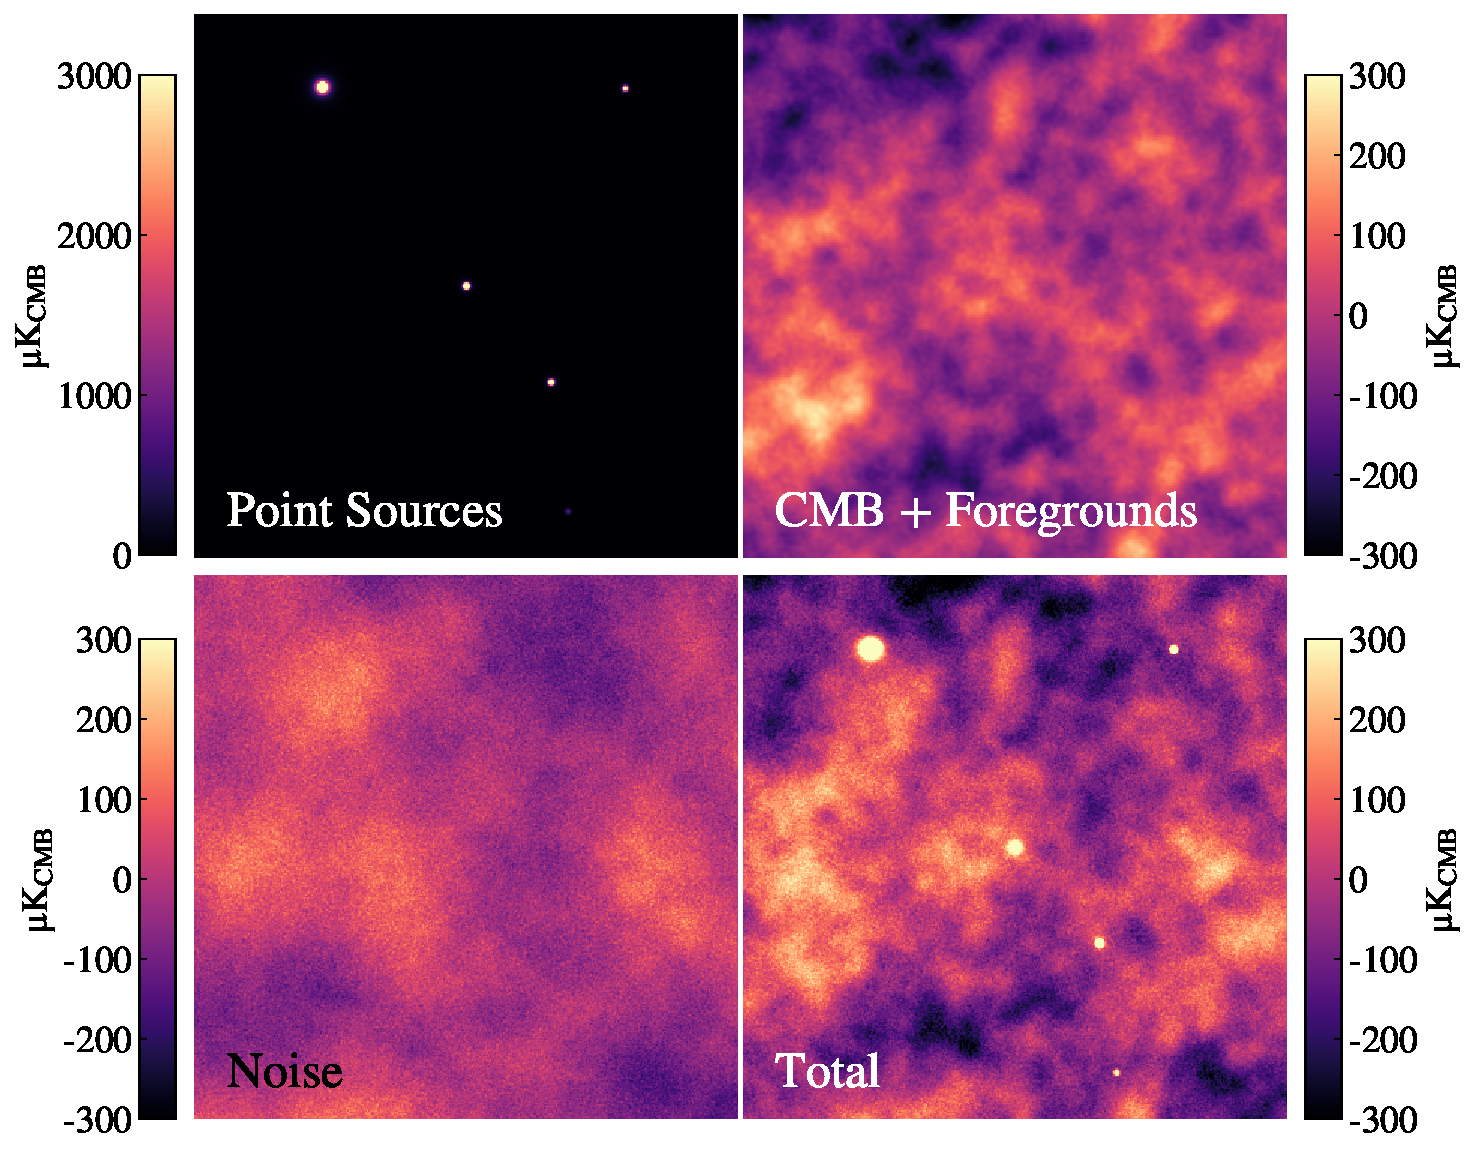
\includegraphics[width=\linewidth]{Figures/simmap.png}
    \caption{Example of a simulated map used to characterize the stacking bias.  This example is for PA5 in the F090, zoomed in to an area of $2\deg\times2\deg$.  Top left: Point-source map using the input catalog RA and DEC coordinates.  Top right:  Simulated CMB.  Bottom left:  Simulated noise~\cite{atkins}.  Bottom right: Final simulated map after combining the previous three components.  This process is done for each PA and F-band, and repeated 100 times to estimate radial profile errors.
    }
    \label{fig:sim_map}
\end{figure*}

We simulate a stacked profile to validate our stacking pipeline and to estimate statistical uncertainty on the radial profiles presented in Section~\ref{sec:act_results}.  We first simulate a map by combining simulated point sources (referencing the catalog) along with a simulated CMB and foregrounds, and additionally adding simulated noise.  An example of a simulated map (box area of $\pm2\deg$ is shown in Figure~\ref{fig:sim_map}.  The four quadrants show the three main components of the simulated maps, followed by the total simulated map as the prior three are combined.  Here, we detail the construction of the simulations.

\subsection{Point Source Map Simulation}
\label{subsec:sim_ptsrc}
A point source map is simulated using the input catalog, and point source selection described in Section~\ref{subsubsec:cat_sel}.  The Uranus-derived beam defines the shape of the point sources in the simulated map.  Fluxes of each point source are obtained from the catalog and converted to the units of the data maps ($\mu K_\text{CMB}$) using the fiducial beam solid angle and center frequency of the passbands.

The fiducial beam profile, fluxes and coordinates are then given to the \verb|pixell.sim_objects| function that outputs a simulated point source map with matching point sources and map shape as the catalog and DR6 map. We choose to apply to the simulated map a pixel window function that matches that of the data maps for ease of comparison.

\subsection{CMB Simulation}
\label{subsec:sim_cmb}
The second component of the simulation is diffuse sky signal comprised of the CMB and (extra-)Galactic foregrounds.  This signal is critical in the simulation because the CMB is a significant source of noise in our stacked profiles at intermediate angular scales.  To accurately estimate the uncertainty and bias introduced by the inpaint-subtraction method described in Section~\ref{subsec:stacking}, we must include the CMB in our simulations.

We use the DR4 $C_\ell^{TT}$ power spectra to draw Gaussian realizations of the diffuse sky signal. An example of this simulated signal is shown in the top right of Figure~\ref{fig:sim_map}.  This simulation also contains foregrounds, which are an important contribution at high multipoles.

\begin{figure*}[t]
    \centering
    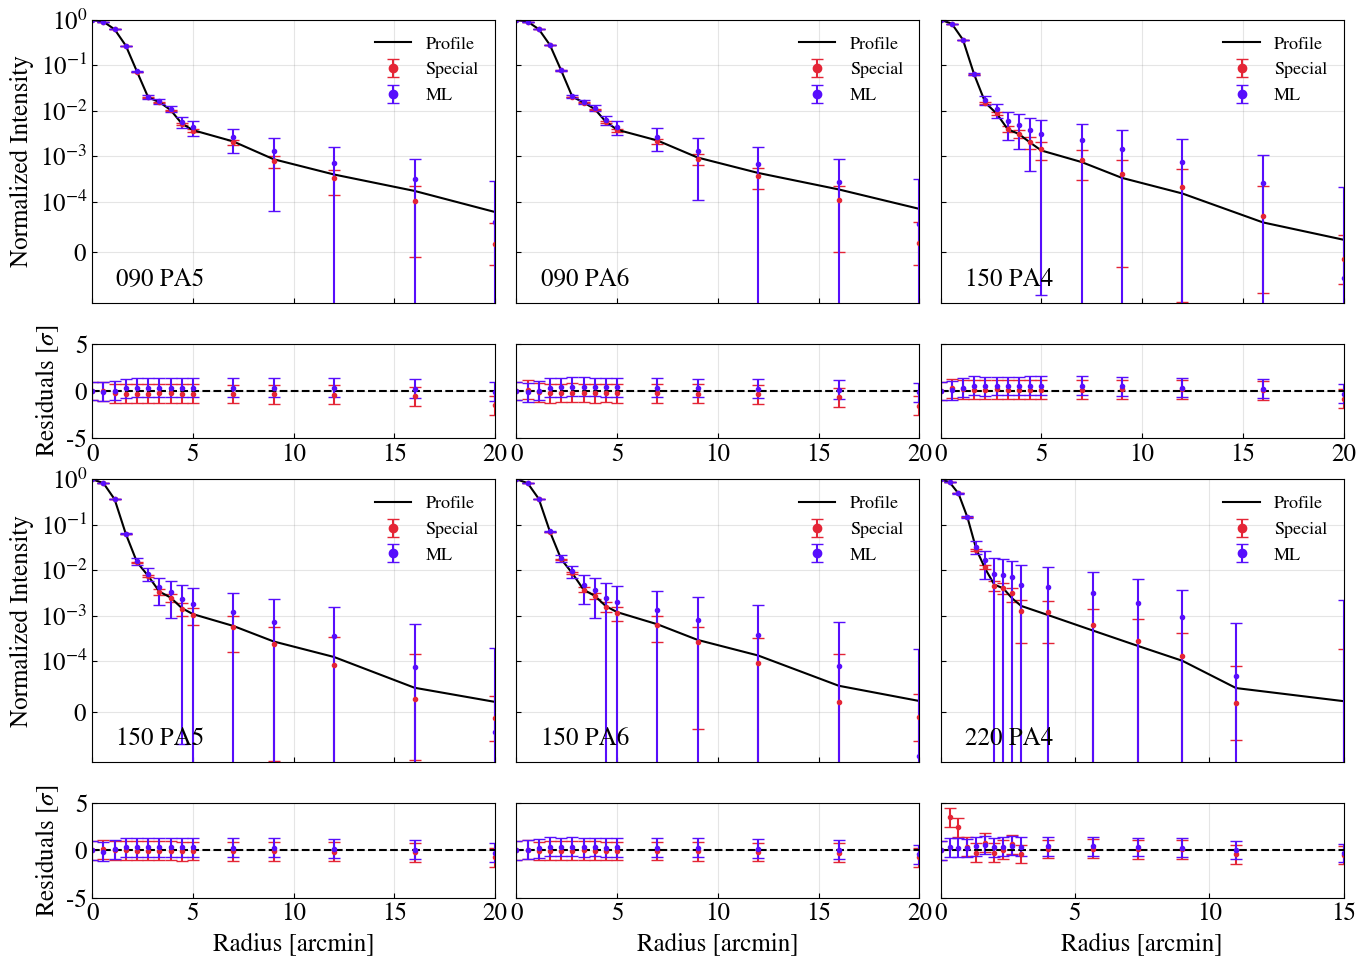
\includegraphics[width=\textwidth]{Figures/profiles_sims.png}
    \label{fig:simprofs}
    \caption{Mean simulated radial profile at each F-band and PA.}
\end{figure*}

\subsection{Noise Simulation}
\label{subsec:sim_noise}
The third component to complete our simulated maps is noise.  The estimation of map noise is twofold: 1) a realization of the ACT map-based noise simulations at large angular scales ($\ell<5000$) and 2) a white-noise realization drawn from the per-pixel variance maps that accompany the DR6 maps.

The ACT map-based noise simulations will be fully described in an upcoming paper accompanying the DR6 release. Noise simulation maps include atmosphere, ACT scan strategy, and a more detailed approach to model correlated instrument noise.  An individual noise simulation is used for each individual simulated map.

As the map-based simulations at the time of this analysis only describe the noise on large angular scales ($\ell<5000$), we manually fill in the noise on small angular scales.  We then splice together two noise simulations in $\ell$-space, such that the white noise term occupies the lower $\ell$-space and map-based noise dominates the high $\ell$-space.  An example patch of the noise map is shown in the bottom left of Figure~\ref{fig:sim_map}.

Figure YYY shows the mean simulated profile at each PA and F-band compared to the Uranus-derived beam.

\section{Results}
\label{sec:act_results}
Here, we detail the resulting temperature and temperature-to-polarization leakage beams acquired from the stacking method described above. 

\begin{figure*}[t]
    \centering
    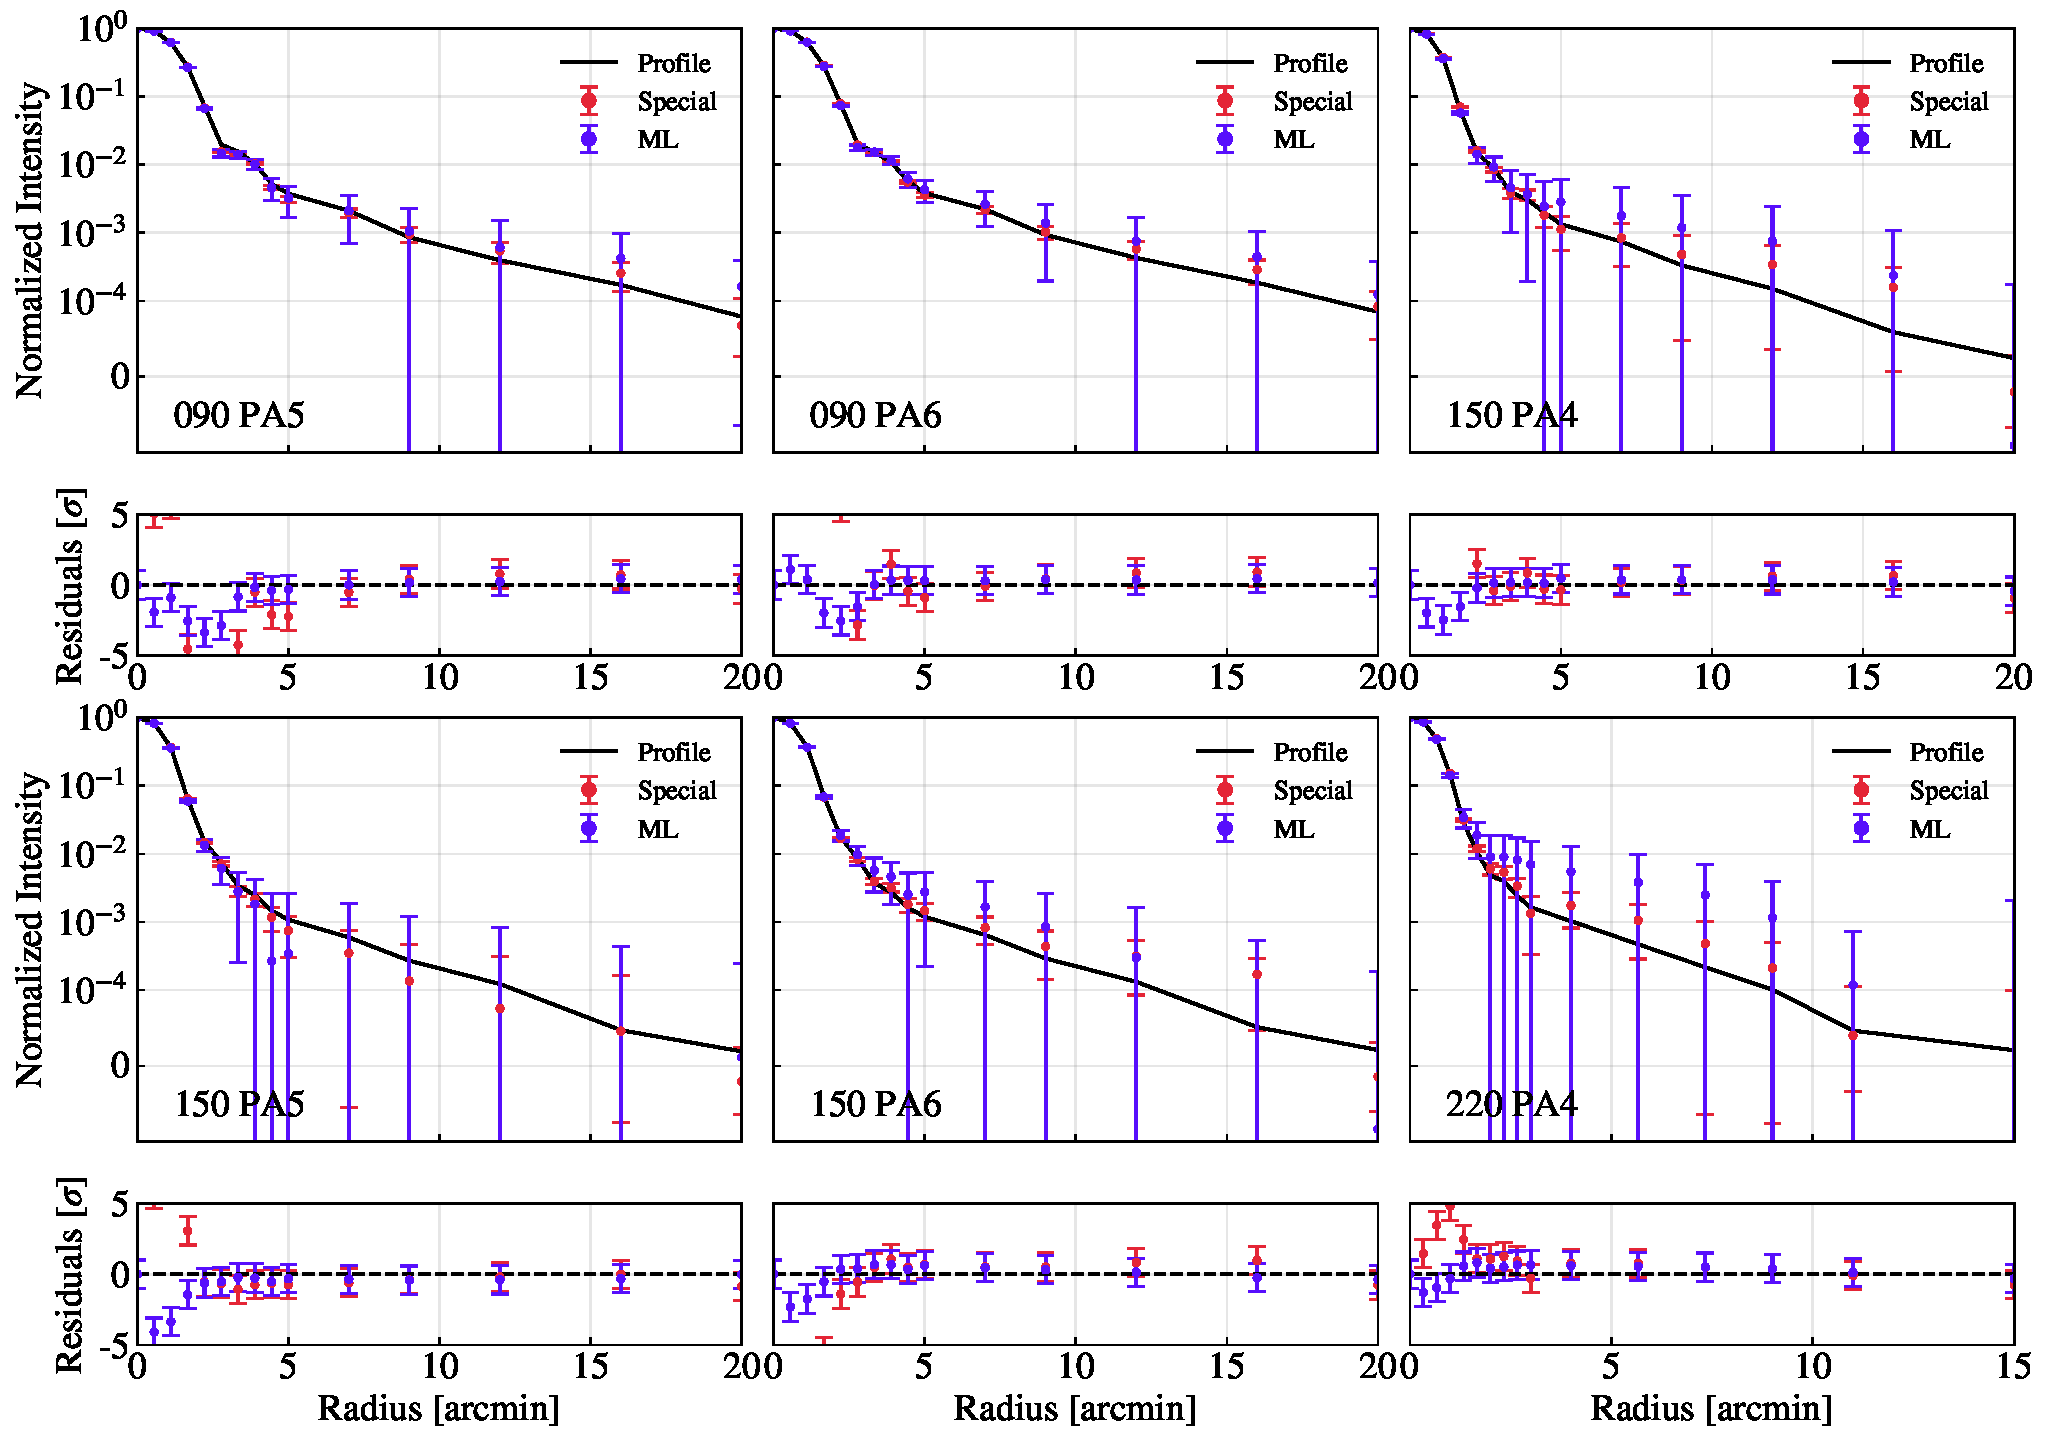
\includegraphics[width=\textwidth]{Figures/profiles_noP_15.pdf}
    \caption{The average radial profile of the simulated observations for PA5 at 150 GHz, comparing the azimuthal averages of the input 2D beam model and the beam of the stacked point sources. 
    }
    \label{fig:profiles}
\end{figure*}

\subsection{Main Beam}
\label{subsec:mainbeam}
This section presents the temperature profiles from stacks and compares them to the existing Uranus-derived beams from Uranus. 
\subsubsection{Profiles}
\label{subsubsec:profiles}
The stacked profiles are shown in Figure~\ref{fig:profiles}.  Each profile shows the Uranus Uranus-derived beam in black, with individual arrays plotted separately.  The bottom panel shows the difference between each array's profile to the planet.
\subsubsection{Spatial Variation}
\label{subsubsec:null_mainbeam}

To study the spatial variation of point sources, we conducted a "null test" where we stacked four categories of point sources: high and low, RA and DEC.  We separate the catalog in half by considering the median RA and DEC, such that the four categories are $\text{RA}_{\text{low}}$, $\text{RA}_{\text{high}}$, $\text{DEC}_{\text{low}}$ and $\text{DEC}_{\text{low}}$ (separated by their median values). 
 Figure~\ref{fig:bells} shows the resulting window functions $B_{\ell}$ for each F-band and PA.

From this test, we find the special sources have spatial dependence where the $\text{DEC}_{\text{low(high)}}$ and $\text{RA}_{\text{high(low)}}$ match in window function, but differ from its opposite.  \textcolor{red}{Sentence explaining this effect or how it is consistent with other analyses.}

\begin{figure*}
    \centering
    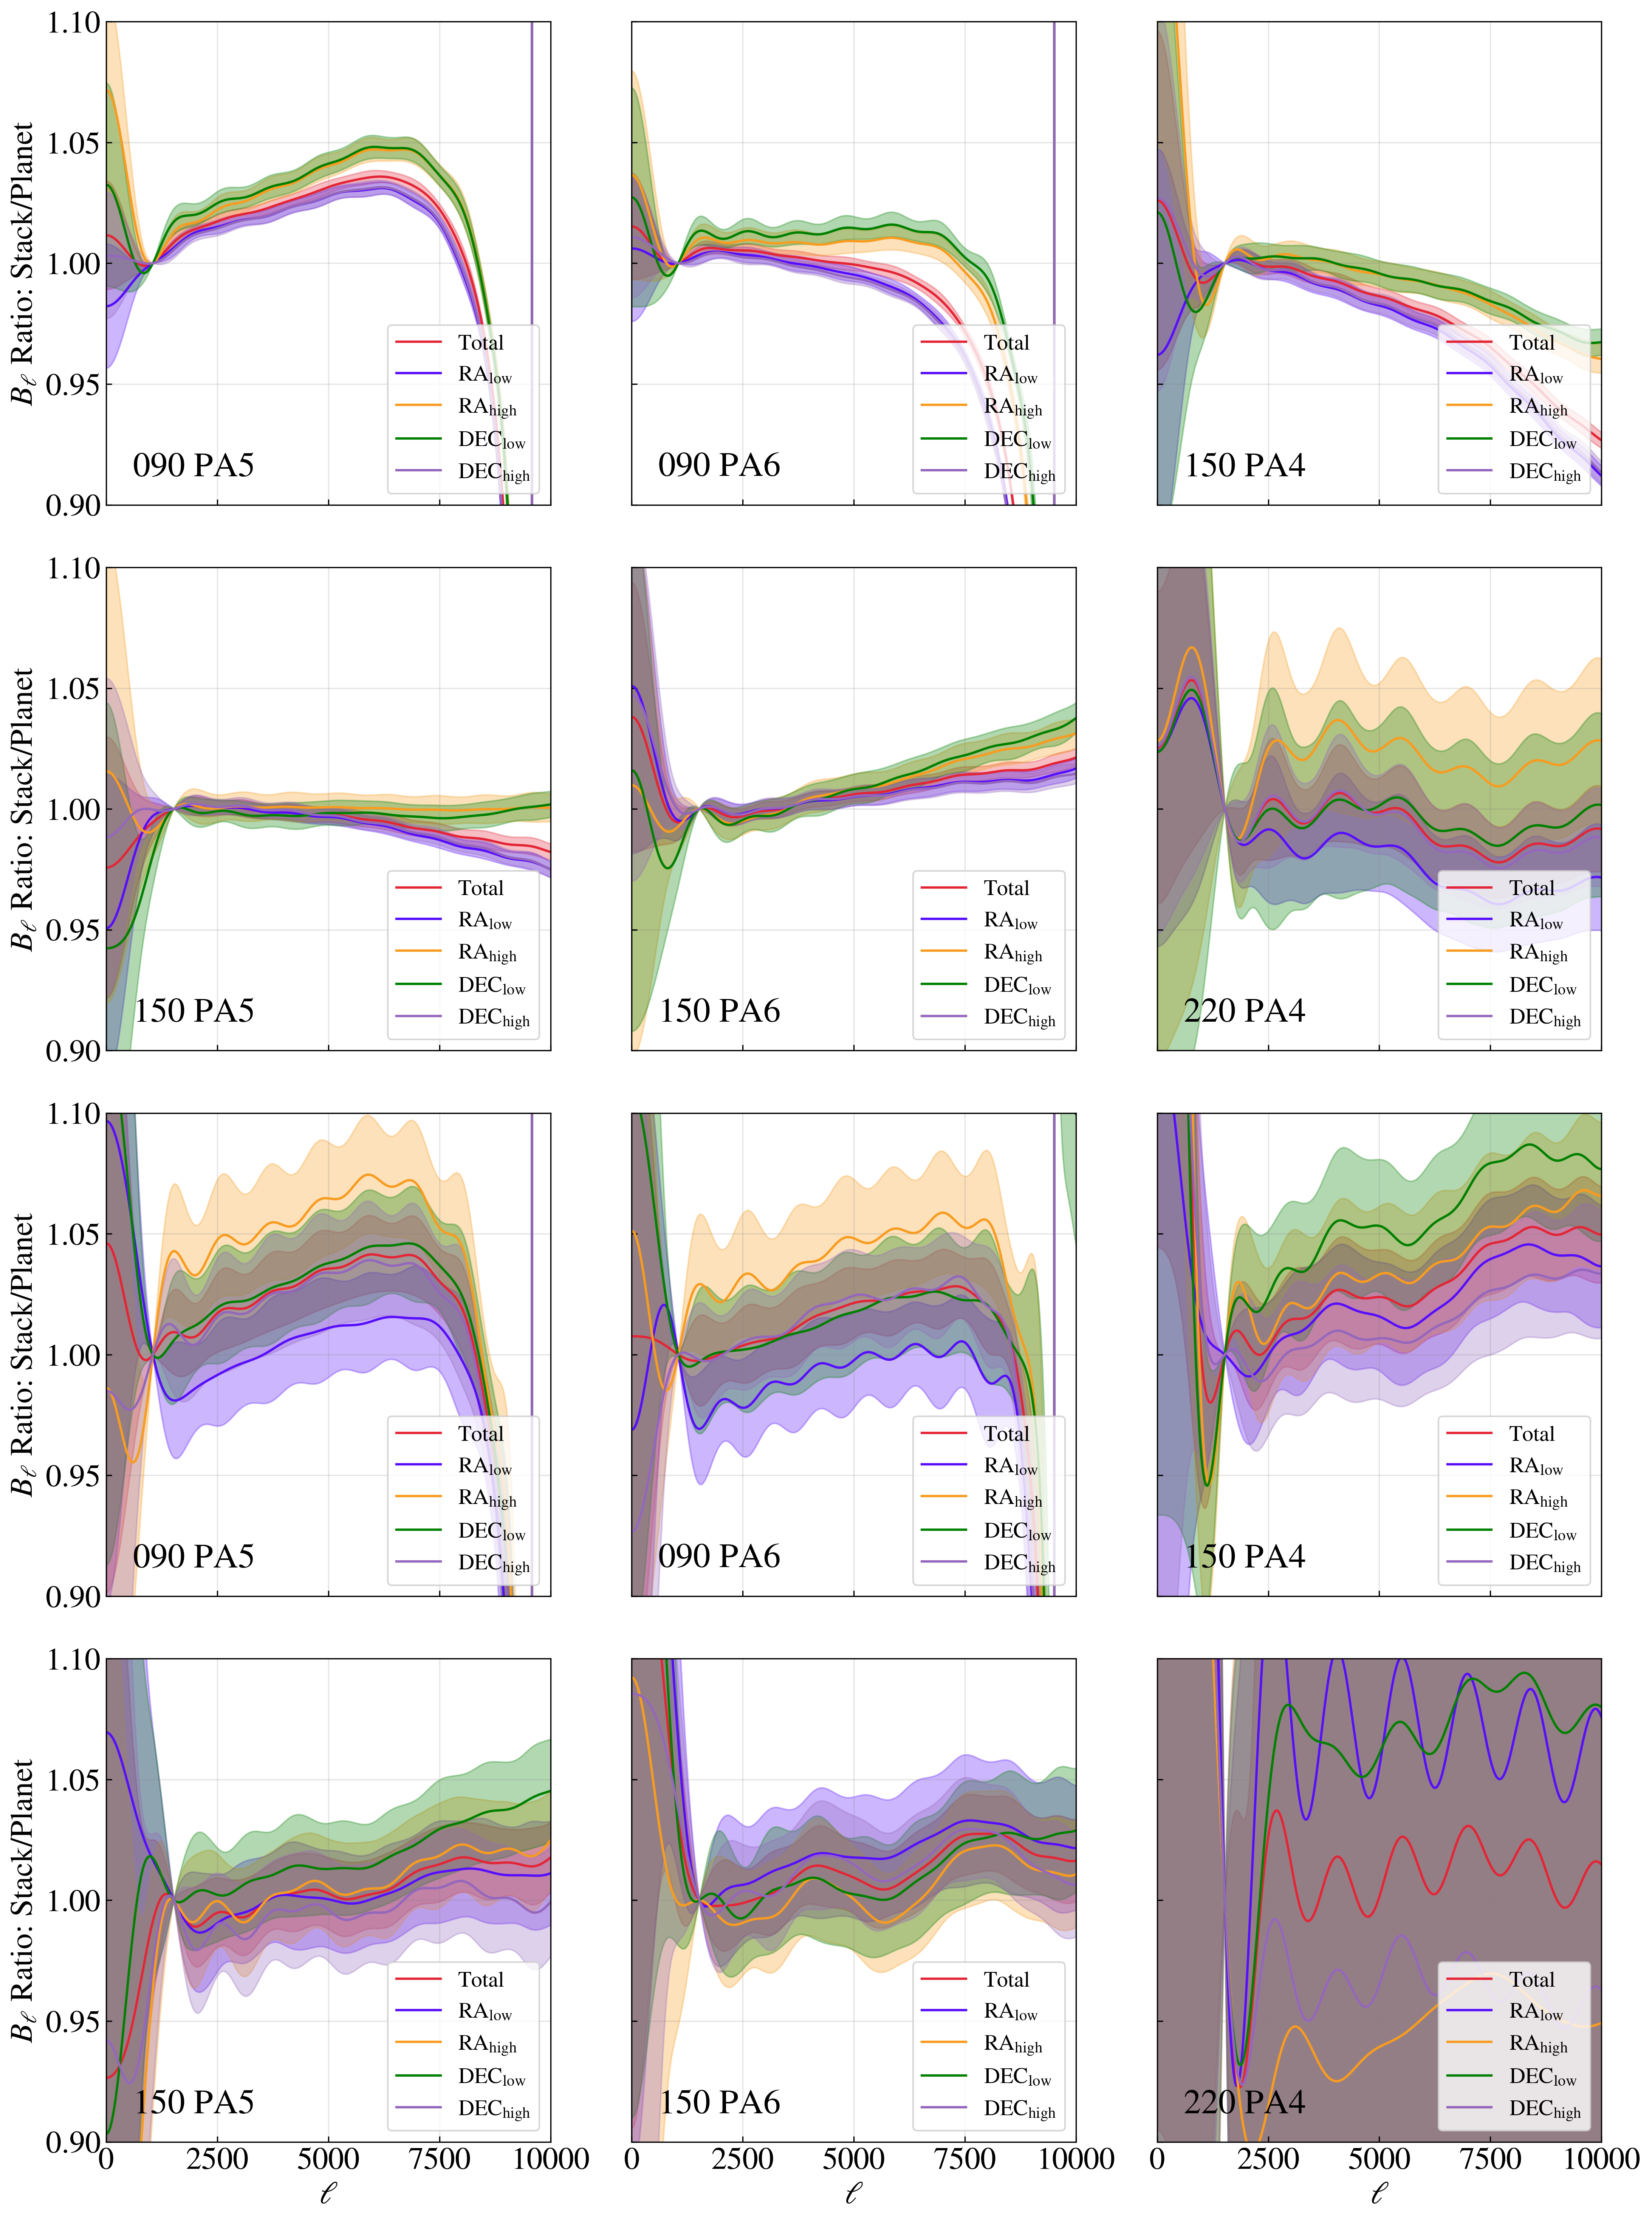
\includegraphics[width=\textwidth]{Figures/Bells_ratio_planet.pdf}
    \caption{Window function of stacked point sources, separated by RA and DEC, which we consider as a null test.  The full map stacked is plotted in red.}
    \label{fig:bells}
\end{figure*}

\subsection{Temperature to Polarization Leakage Beam}
\label{subsec:polbeam}

Here, we present the polarized beams of the stacked point sources to determine polarization leakage in the instrument.  The leakage is relatively small compared to the magnitude of the temperature beam, however the sensitivity of ACT DR6 data is such that this leakage needs to be accounted for in the analysis.  Previously, observations of Uranus were used to build an $\ell$-space T-to-P leakage function for a given frequency and array in the instrument.  Here, we test this method by comparing the leakage to our new method of stacking.

\begin{figure*}[t]
    \centering
    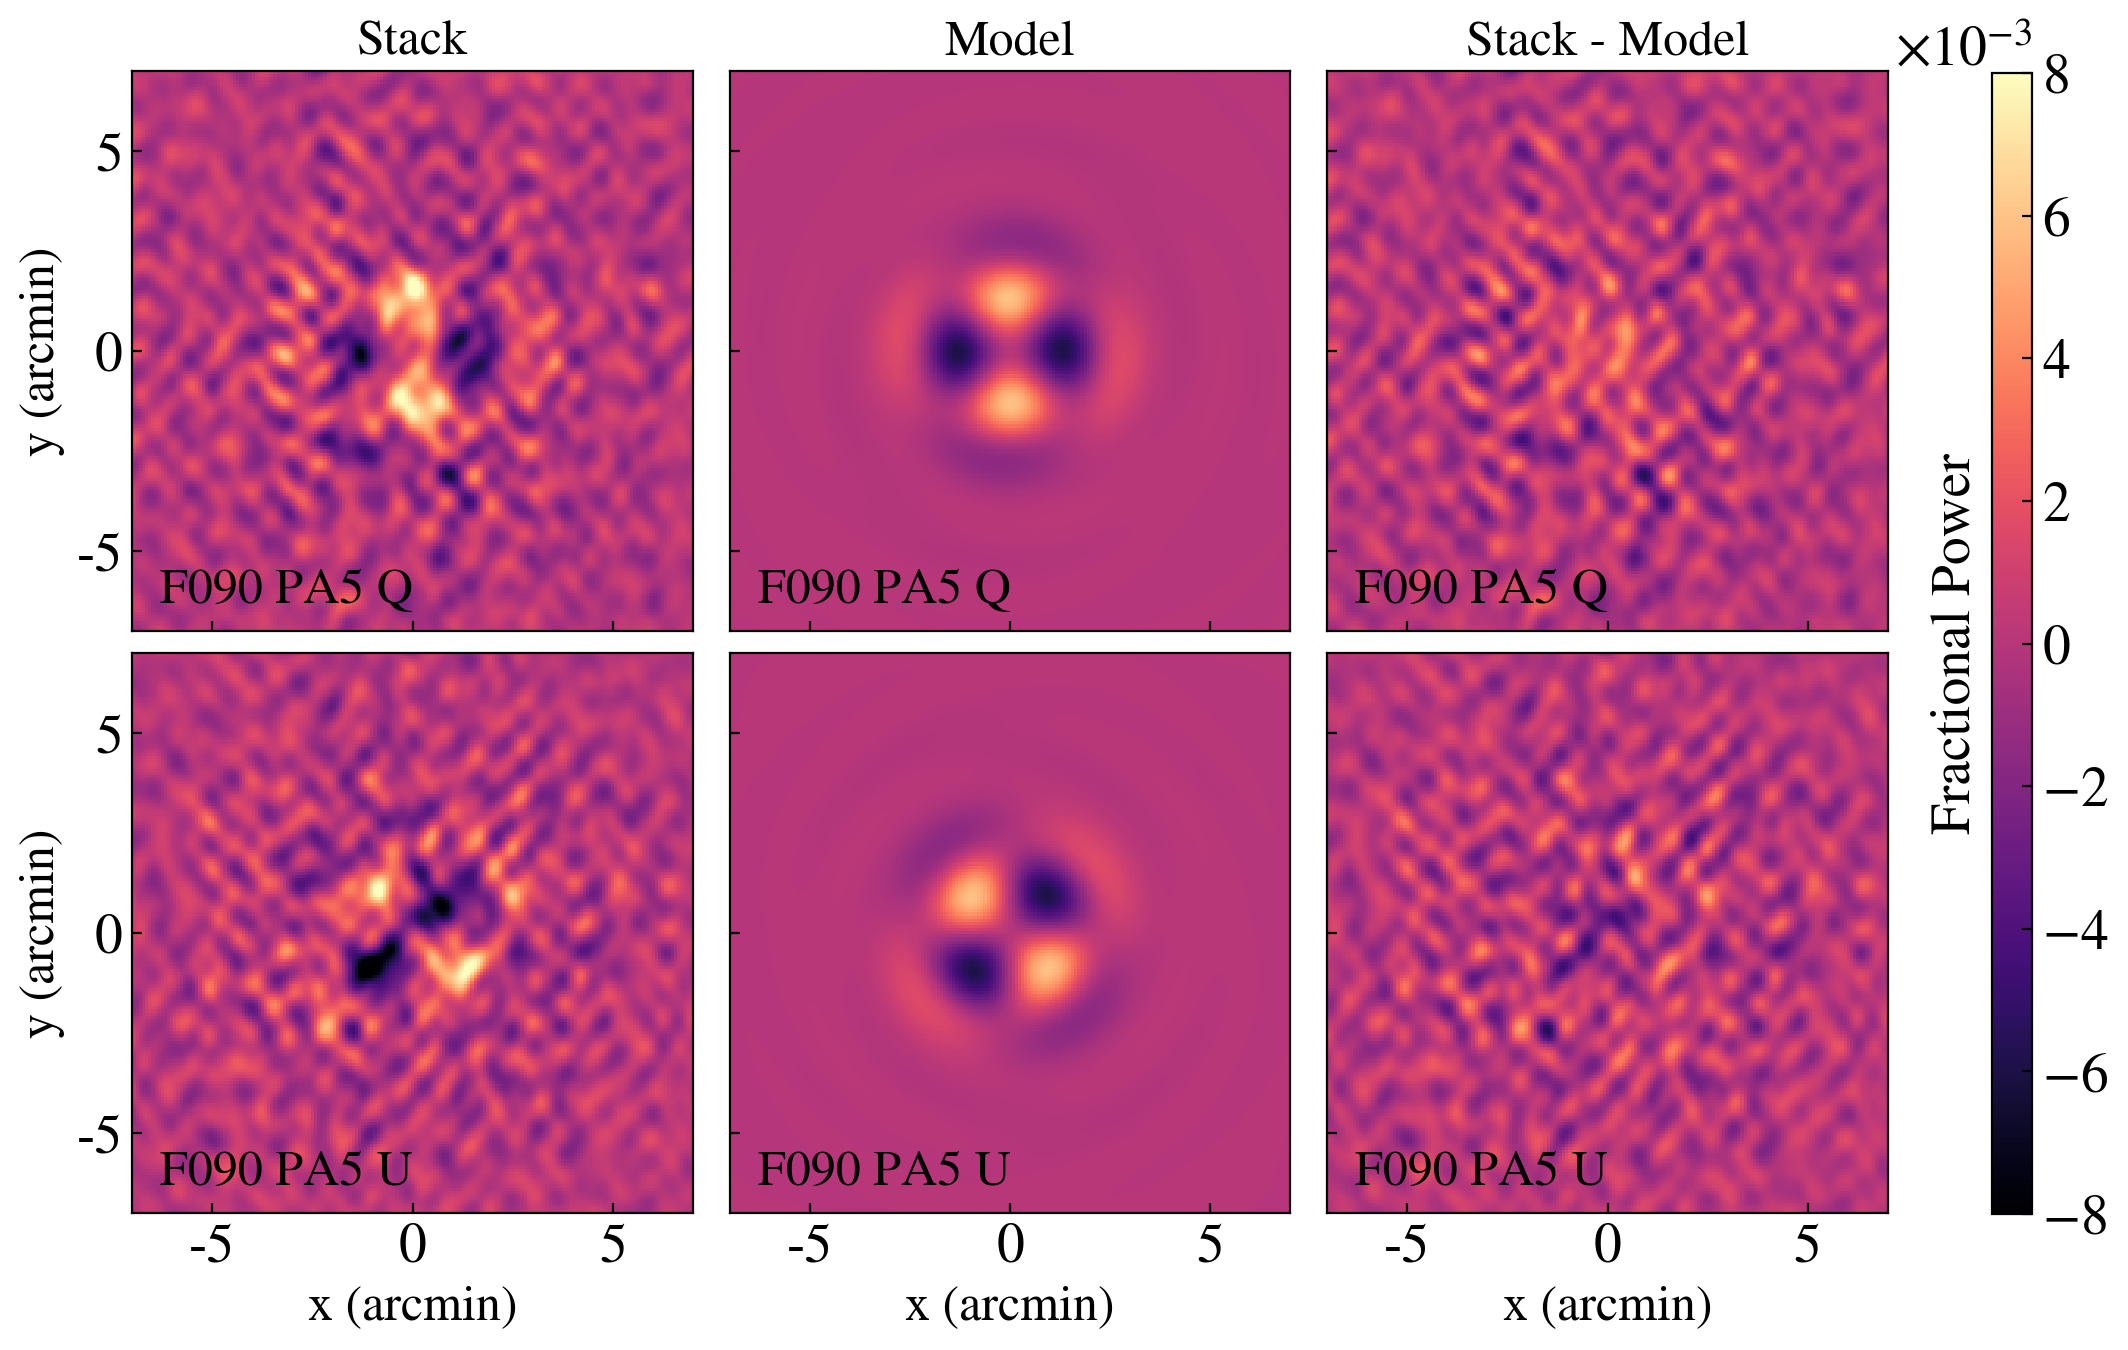
\includegraphics[width = \textwidth]{Figures/polbeams.png}
    \caption{Polarization leakage from stacked F150 PA4 beam, for the ML sources.  The left column shows the stacked map, the middle column is the modeled polarization leakage, and the right column is the difference between them.}
    \label{fig:polmodel}
\end{figure*}



\begin{figure*}
    \centering
    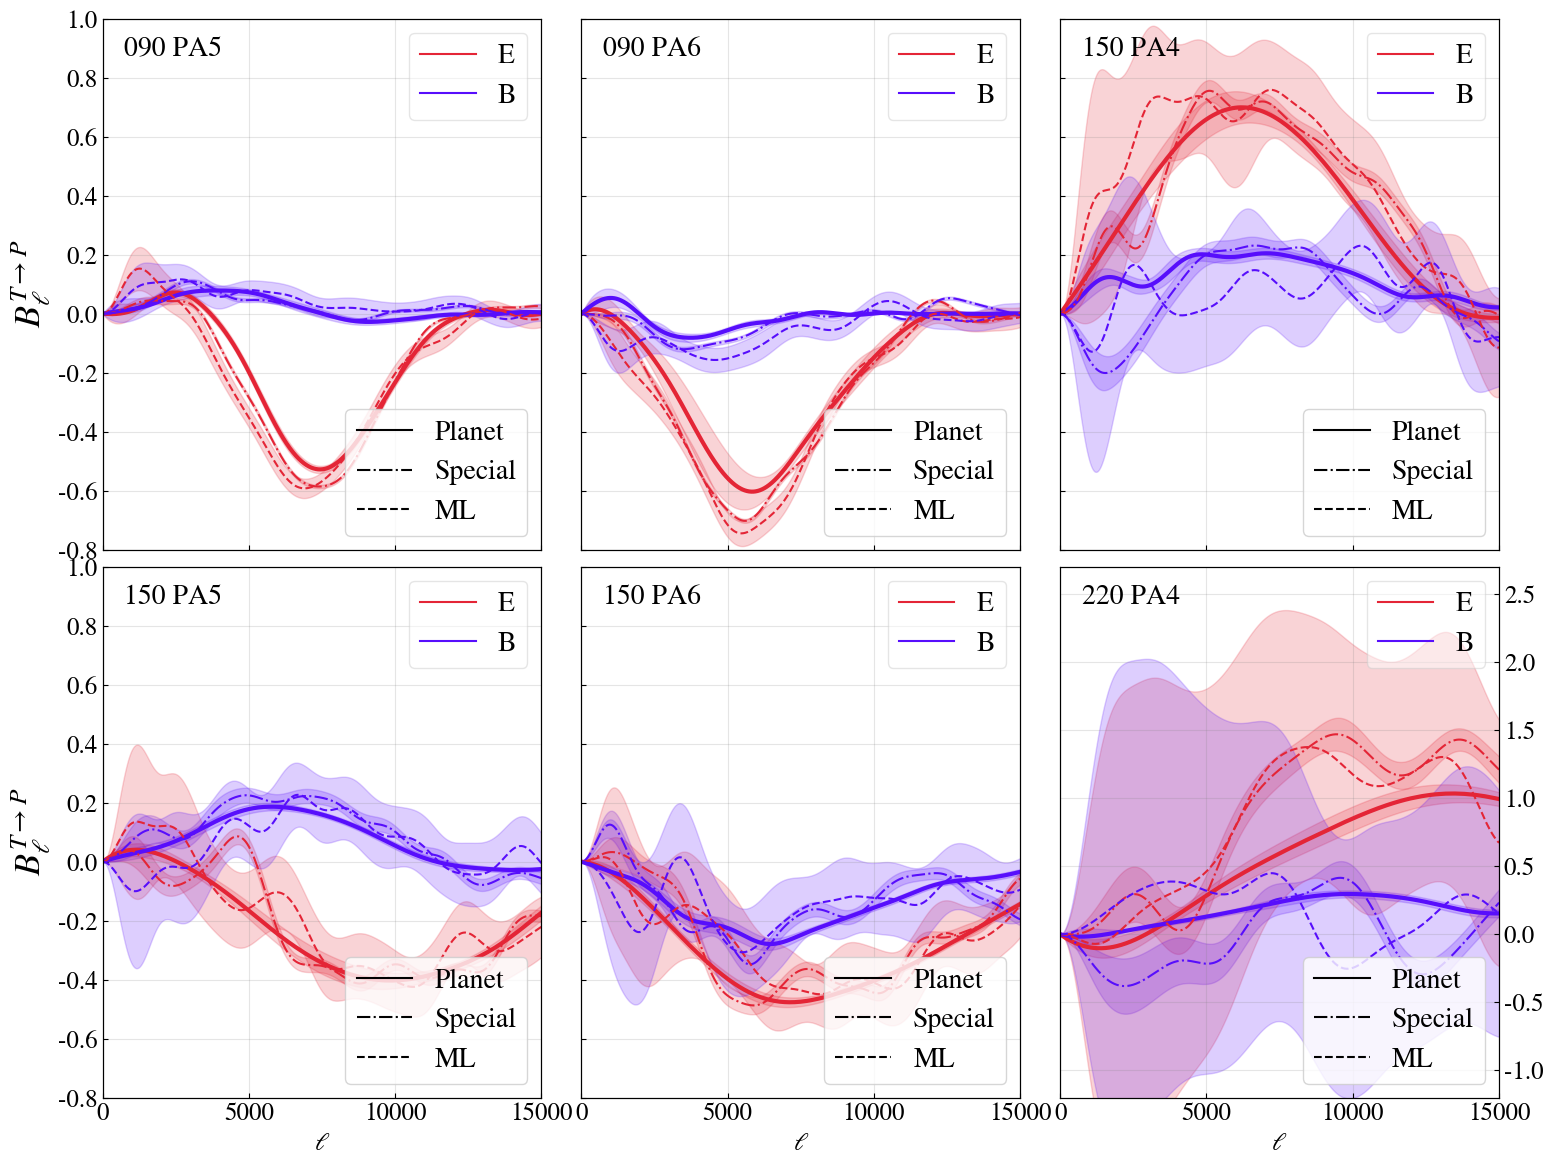
\includegraphics[width = \textwidth]{Figures/leakage.pdf}
    \caption{Polarization leakage from stacked}
    \label{fig:leakage}
\end{figure*}

Figure~\ref{fig:polmodel} shows an example of the stacked polarization leakage beam, the modeled beam, and the residual for F150 PA4. Note that the quadrupole shape of the model is due to the reprojection to the stack geometry: although we model the leakage beam as azimuthally symmetric when located on the pole of the standard spherical coordinate system, the symmetric shape turns into a quadrupole shape when rotated to the stack geometry location, which is centered on the equator. From the window functions, we obtain the window functions of each array's T$\xrightarrow[]{}$E and T$\xrightarrow[]{}$B leakage (Figure~\ref{fig:leakage}).


\section{Discussion}
\label{sec:act_disc}

\subsection{Beam Products}
\label{subsec:prods}

\subsection{Conclusion}
\label{subsec:concl}
In this paper, we have presented the analysis of the ACT beams for DR6, which includes data from 2017--19. ...